\documentclass{article}
\usepackage{graphicx}
\usepackage[margin=1.5cm]{geometry}
\usepackage{amsmath}

\begin{document}

\title{Monday Reading Assessment: Unit 4, Sources of Magnetic Fields}
\author{Prof. Jordan C. Hanson}

\maketitle

\section{Memory Bank}

\begin{itemize}
\item $\oint \vec{B} \cdot d\vec{l} = \mu_0 I_{\rm enc}$ ... Amp\`{e}re's Law
\item $\vec{B} = \mu_0 (N/L) I_{\rm enc} \hat{z}$ ... \textit{Solenoid B-field.}
\item $\vec{B} = \mu_0 I / (2\pi r)$ ... B-field of a wire a distance $r$ away from it.
\end{itemize}

\begin{figure}[ht]
\centering
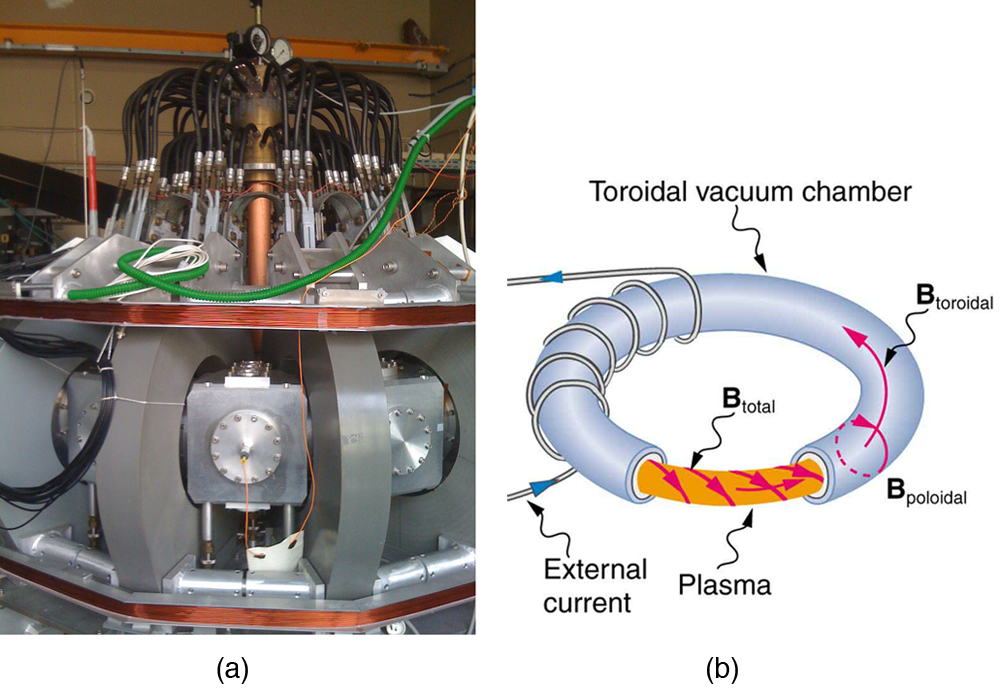
\includegraphics[width=0.35\textwidth,trim=8.5cm 1cm 0cm 3cm,clip=true]{toroid.jpeg}
\caption{\label{fig:fields} A basic diagram of a \textit{toroid}, which is a solenoid wrapped into a circular tube.}
\end{figure}

\section{Solenoids and Toroids}

\begin{enumerate}
\item What is the B-field inside a solenoid with 1000 turns per meter, carrying a current of 10 A? \\ \vspace{1cm}
\item Consider Fig. \ref{fig:fields}.  Suppose the current is 10 Amps, and the number of total turns is 4000.  If the radius of the toroid in Fig. \ref{fig:fields} is 2 meters, what is the toroidal B-field inside of it? \\ \vspace{2cm}
\item Suppose plasma is trapped inside the toroid, and has an effective current of 0.1 Amp.  What is the \textit{poloidal} field that results from this current, at a distance of 0.5 m from the center of the plasma, corresponding to the radius of the pipe?
\end{enumerate}

\end{document}
